\apendicemanual{Protótipos da interface do Memora}{ap:capturas-complementares}
As telas representam o projeto elaborado no Figma, anterior à implementação dos comportamentos da aplicação. A análise por acesso prevista na etapa Analisar foi incorporada ao histórico da etapa Simular.

\begin{figure}[!htbp]
\centering
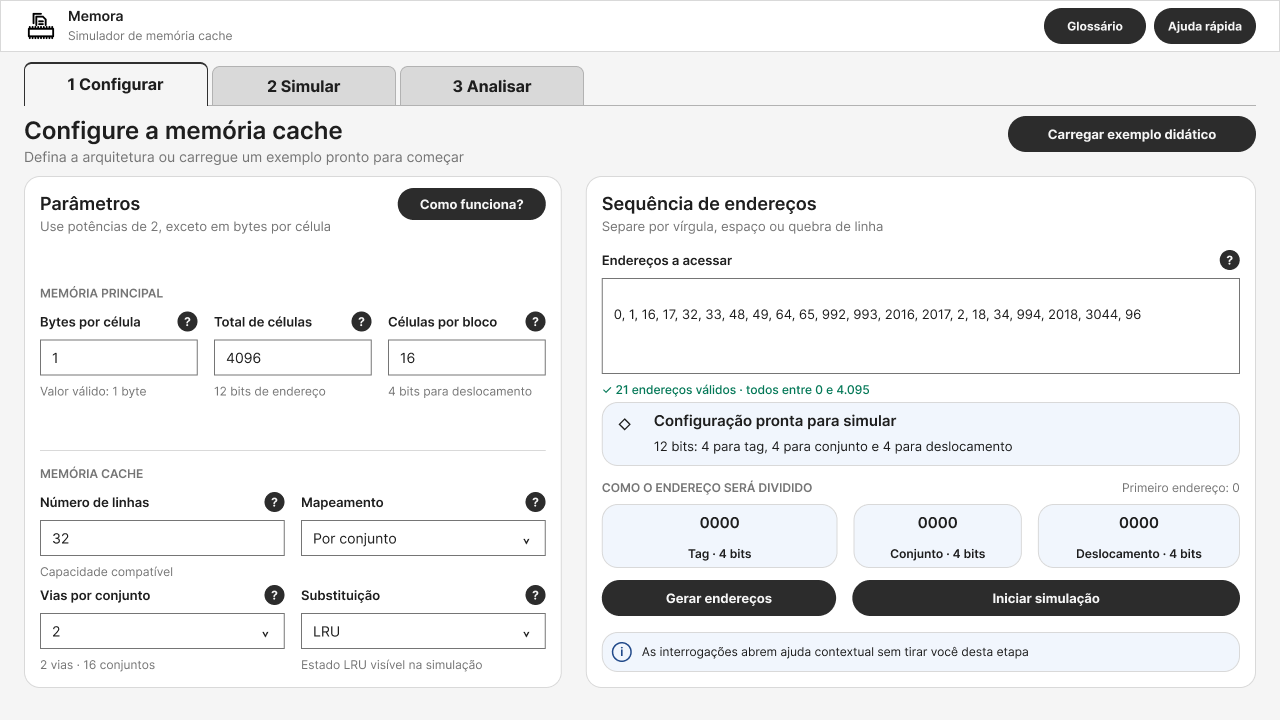
\includegraphics[width=\linewidth,height=.35\textheight,keepaspectratio]{figuras/figma-configurar.png}
\caption{Protótipo da etapa Configurar no Figma.}
\label{fig:figma-configurar}
\par\footnotesize Fonte: elaboração própria no Figma.
\par\bigskip

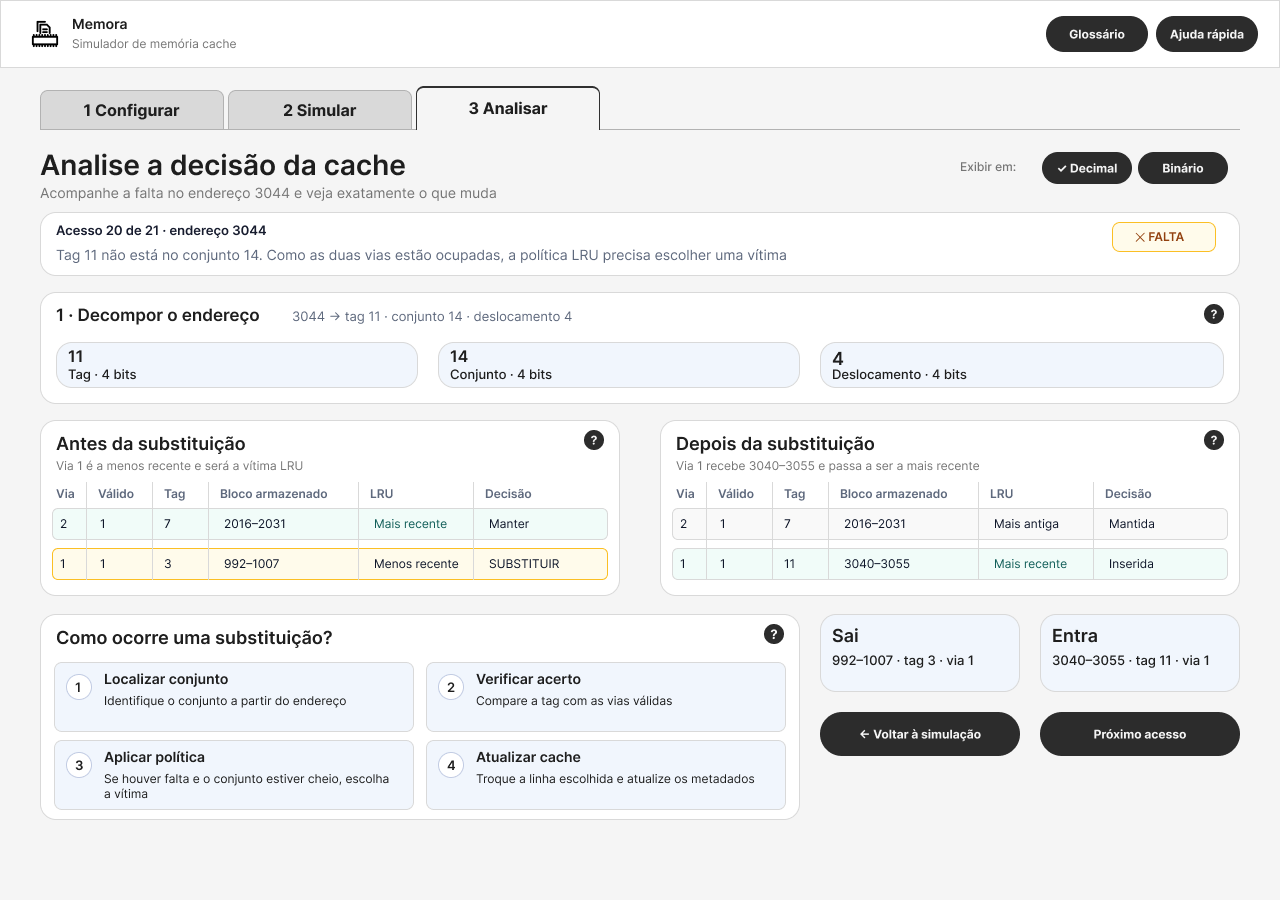
\includegraphics[width=\linewidth,height=.35\textheight,keepaspectratio]{figuras/figma-analisar.png}
\caption{Protótipo da análise de um acesso, antes da integração ao histórico.}
\label{fig:figma-analisar}
\par\footnotesize Fonte: elaboração própria no Figma.
\end{figure}

